\documentclass[11pt]{article}

% Change "review" to "final" to generate the final (sometimes called camera-ready) version.
% Change to "preprint" to generate a non-anonymous version with page numbers.
\usepackage[review]{acl}

% Standard package includes
\usepackage{times}
\usepackage{latexsym}

% For proper rendering and hyphenation of words containing Latin characters (including in bib files)
\usepackage[T1]{fontenc}

% This assumes your files are encoded as UTF8
\usepackage[utf8]{inputenc}

% This is not strictly necessary, and may be commented out,
% but it will improve the layout of the manuscript,
% and will typically save some space.
\usepackage{microtype}

% This is also not strictly necessary, and may be commented out.
% However, it will improve the aesthetics of text in
% the typewriter font.
\usepackage{inconsolata}

%Including images in your LaTeX document requires adding
%additional package(s)
\usepackage{graphicx}

% Added for this manuscript
\usepackage{amsmath}
\usepackage{amssymb}
\usepackage{booktabs}
\usepackage{multirow}
\usepackage{xcolor}
\usepackage{array}

\newcommand{\boxedtok}{\texttt{\textbackslash boxed\{\}}}
\newcommand{\eop}{\texttt{<End\_of\_Prefix>}}
\newcommand{\sd}[1]{$_{\pm #1}$}

\title{Decisive, Not Difficult: Allocating Learning Effort\\across Reasoning Steps in Long-CoT Distillation}

\author{First Author \\
  Affiliation / Address line 1 \\
  \texttt{email@domain} \\\And
  Second Author \\
  Affiliation / Address line 1 \\
  \texttt{email@domain} \\}

\begin{document}
\maketitle
\begin{abstract}
Long chain-of-thought (CoT) distillation methods decide which traces, steps or tokens a student learns from, mostly through hard thresholds, and then weight what they keep uniformly.
We study how supervision should instead be \emph{allocated} across the steps of fixed teacher traces.
We weight each step by its \emph{answer-information gain}: the change in the frozen student's log-probability of the gold answer when the step is appended, scored offline with cached teacher-forced probes (12 GPU-minutes for 966 traces).
The gains are standardized within each trace and turned into weights normalized so that every trace keeps its total token weight; no step is removed.
A shuffled control shows that entropy-based weights, from a signal that orders steps almost like spectral gradient strength and step loss, are matched by the same entropy scores shuffled within each trace.
Distilling DeepSeek-R1-Distill-Qwen-1.5B on 966 public traces, answer-gain allocation raises average pass@1 on AIME24, AIME25, AMC12 and MATH500 from 41.65 to 42.46 (+0.82) over uniform training in the same pipeline, and is above it on both pass@1 and pass@3 under each of three sampling seeds of one training run; on pass@3 it ties the entropy and shuffled controls.
\end{abstract}

\section{Introduction}

Small reasoning models are commonly obtained by supervised fine-tuning (SFT) on long CoT traces written by a stronger model \citep{deepseek2025r1}.
These traces run to thousands of tokens and mix steps of very different value: restatements, hedges, self-checks, abandoned attempts, and the few steps that decide the answer \citep{bogdan2025thoughtanchors}.
Plain SFT gives every token the same weight.

Recent work improves on this by deciding \emph{what} the student learns.
Some methods build better traces: s1 \citep{muennighoff2025s1} and LIMO \citep{ye2025limo} curate about a thousand traces, and CoRD \citep{yun2026cord} assembles traces step by step from several teachers, keeping the candidates under which a 32B meta-prover finds the gold answer most likely.
Others adapt traces to the student: P-ALIGN \citep{liu2026palign} keeps the shortest teacher prefix the student judges sufficient and lets the student write the rest, and step-entropy compression \citep{li2026stepentropy} and SPIRIT \citep{cui2025spirit} delete low-information steps.
Others select what enters the loss: SGL \citep{fan2026sgl} keeps the steps whose gradients load on a low-rank consensus subspace, and Segment-Selective SFT \citep{wang2026segattr} keeps segments with high integrated-gradient attribution toward the answer; Reasoning Scaffolding \citep{wen2026scaffolding} adds an auxiliary task instead.

\paragraph{What these methods leave open.}
First, their decisions are binary and hinge on thresholds, such as SGL's 95\% energy, Segment-Selective SFT's attribution share and consistency cut (set by search to $0.7$ and $0.8$) and the 80\% pruning ratio of step entropy.
A step on either side of the cut is learned fully or not at all: on the traces we study, SGL's gate removes 41\% of response tokens, including the step that writes the final answer in 37\% of traces, and scores below plain SFT (\S\ref{sec:iwc-test}).
Second, the content they keep is trained uniformly, so a restatement and the derivation of the answer receive the same weight.
Soft objectives do reweight supervision (\S2), but per token and by the model's own confidence or gradient utility, not per step and by how much a step advances the answer.
Third, their signals are tied to their pipelines and often costly: a 32B meta-prover during generation, integrated gradients, student generations and self-judgments, or LLM-labeled signals.

\begin{figure*}[t]
  \centering
  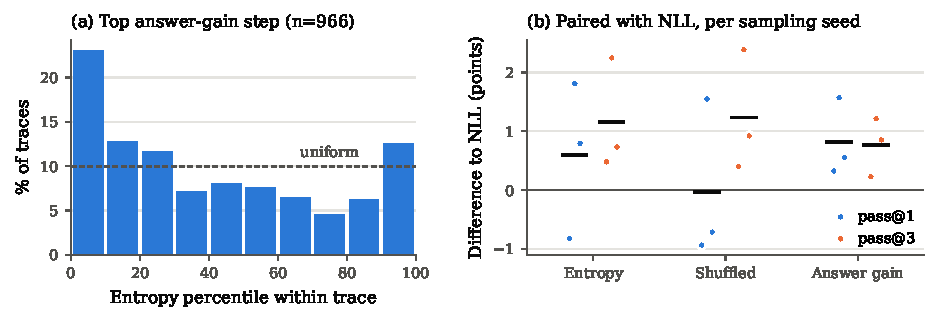
\includegraphics[width=\textwidth]{figures/figure1.pdf}
  \caption{(a) Within-trace entropy percentile of the step with the largest answer gain, excluding steps that write \boxedtok{}. Mass concentrates on low-entropy steps: 63\% lie below the median. (b) Difference to uniform training (NLL) of each allocation, one dot per sampling seed of one training run; bars mark the mean. Only answer gain is positive on all six comparisons.}
  \label{fig:main}
\end{figure*}

\paragraph{This paper.}
We allocate supervision across the steps of fixed traces by \emph{answer-information gain}: the change in the frozen student's log-probability of the gold answer when a step is appended, read through a fixed answer probe.
Steps with high gain are what we call \emph{decisive}.
The quantity is not new as a credit signal \citep{ton2025infogain}; what we contribute is its use as an offline, step-level supervision weight in distillation.
Unlike CoRD's score, it measures the \emph{change} a step causes rather than the level it reaches, and it is read from the student itself rather than from a larger model.
We turn gains into weights by standardizing them within each trace and normalizing so that every trace keeps the total token weight it has under uniform SFT.
A weight acts as a soft threshold: no step is cut, every step keeps at least half of its uniform weight, and hard selection is a limiting case (\S\ref{sec:objective}).
Because the weights act only on the loss, they can be added to the trace sources and masks above (\S\ref{sec:compose}).

\paragraph{Evidence.}
We test allocation with the data, model, recipe and evaluation fixed and shared with the baselines above, on the 966 public traces released by \citet{liu2026palign}, which serve only as a testbed: the method uses none of P-ALIGN's machinery.
Answer-gain allocation raises average pass@1 by +0.82 over uniform training in the same pipeline (42.46 against 41.65) and is ahead of it on both pass@1 and pass@3 under each of three sampling seeds of one training run (Figure~\ref{fig:main}b); on pass@3 it ties the controls.
We arrived at answer gain after the difficulty signals failed.
Step entropy, spectral gradient strength and step loss order the steps of a trace almost identically, and allocating by entropy is matched by a control that step-weighting papers rarely report: the same entropy scores shuffled within each trace (\S\ref{sec:iwc-test}).
Answer gain shows no systematic association with these signals, and the step it ranks highest is usually a low-entropy one (Figure~\ref{fig:main}a).
One explanation, which we offer as a hypothesis, is that a small student learns from information it can \emph{use} \citep{xu2020usable}, and a predictable calculation can create it although its entropy is low.

Our contributions are:
\begin{itemize}
  \setlength\itemsep{0pt}
  \item \textbf{Answer-gain allocation for distillation.} We weight the steps of fixed traces by the frozen student's answer-likelihood gain, with gains standardized within each trace and weights normalized by token mass, so that every token stays supervised and every trace keeps its total weight. The scores are computed offline without sampling, gradients or step-level labels beyond the gold answer, and the weights compose with other trace sources and selective masks (\S\ref{sec:method}).
  \item \textbf{A shuffled control for step weighting.} Entropy, spectral strength and loss order steps alike, and allocating by entropy is matched by shuffled entropy scores; none of the gated configurations we tried beats uniform training (\S\ref{sec:iwc-test}).
  \item \textbf{Results under a shared protocol.} Answer-gain allocation improves pass@1 over uniform training in the same pipeline by +0.82, is ahead on every sampling seed, and has the highest pass@1 among the compared methods; we state its limits, including untested training-seed variance (\S\ref{sec:results}).
\end{itemize}

\section{Related Work}

\paragraph{What to learn.}
Beyond the methods in \S1, EDIT \citep{dai2024edit} finds key steps by contrasting dual CoTs, and KPOD \citep{feng2024kpod} learns token masks from an answer-prediction loss.
Rho-1 \citep{lin2024rho1} keeps tokens with high excess loss against a reference model, and critical-token fine-tuning \citep{ruan2025criticaltoken} keeps tokens whose substitution flips correctness.
Like the curation, adaptation and selection methods above, they decide which content is trained on and weight it uniformly; allocation can be applied on top of any of them.

\paragraph{Soft reweighting.}
Soft objectives reweight tokens instead of removing them.
VCORE \citep{gong2026vcore} reweights tokens by gradient utility.
% TODO: verify whether VCORE's weights are normalized per trajectory; if so, state that its normalization resembles ours.
DFT \citep{wu2026dft} scales each token's loss by its detached probability, and ASFT, DEFT and TrimSFT \citep{zhu2026asft,wang2026deft,jia2026trimsft} anchor, generalize or trim this gate; such objectives help only when the model is already strong \citep{li2026beyondll}.
iw-SFT \citep{qin2025iwsft} reads SFT on curated data as a bound on an RL objective, and Step Rejection Fine-Tuning \citep{slinko2026srft} scores steps with teacher rollouts.
The sampling-free signals in this group measure confidence or gradient utility, and none is compared with a shuffled-weight control.

\paragraph{Answer-likelihood step credit.}
The quantity we allocate by is not new; its use as an offline distillation weight is, as far as our search found.
\citet{ton2025infogain} define step-wise information gain as the drop in cross-entropy of the correct answer after a step, and use it to evaluate CoT.
Answer likelihood or its change also serves as a process reward for RL \citep{wang2026mig,tao2026trace}, as step credit in on-policy self-distillation \citep{li2026dcsd}, and, estimated from sampled completions, as a label for process reward models \citep{royer2026mcnig}.
In distillation, CoRD \citep{yun2026cord} ranks candidate steps by the answer likelihood a 32B meta-prover reaches after them, and Segment-Selective SFT \citep{wang2026segattr} attributes the answer to segments with integrated gradients; both use the score to select.
None allocates learning effort over fixed traces by the change in the student's own belief in the answer.

\paragraph{Usable information.}
$\mathcal{V}$-information \citep{xu2020usable} is the information a bounded predictor family can extract, and unlike Shannon information it can be created by computation; PVI \citep{ethayarajh2022pvi} is its pointwise form.
Answer gain is related in spirit, but it is a likelihood difference under one frozen model and one probe, not an optimum over a predictor family.

\section{Selection and Allocation}
\label{sec:iwc}

A training example is a prompt $x$ and a response $y$.
A segmentation rule (\S\ref{sec:setup}) splits $y$ into \emph{steps} $s_1,\dots,s_K$: contiguous spans of tokens with lengths $\ell_1,\dots,\ell_K$.
A step is the unit we weight; it may contain several operations or ideas.
We write $t\in s_k$ for the token positions of step $k$.
A step-level distillation objective is
\begin{equation}
  \mathcal{L}=-\frac{1}{Z}\sum_{k=1}^{K} M_k\,w_k\sum_{t\in s_k}\log p_\theta(y_t\mid x,y_{<t}),
  \label{eq:iwc}
\end{equation}
where $Z$ counts the tokens with $M_k=1$.
\emph{Selection} sets the mask $M_k\in\{0,1\}$ and decides what is learned.
\emph{Allocation} sets the weight $w_k>0$ of each kept step and decides how much of the supervision it receives.
Uniform SFT uses $M_k=w_k=1$.
Data-side methods select before training, by keeping, deleting or rewriting steps; objective-side methods set $M_k$ in the loss.
The hard selectors in \S2 set $M_k$ and keep $w_k=1$ on what they keep; soft reweighting methods such as DFT instead change the loss coefficient, usually per token rather than per step.

\paragraph{Hard selection by a threshold.}
SGL is a representative objective-side selector, and the one we test.
It scores each step by its \emph{spectral strength}, the average leverage of the step's tokens on the dominant subspace of the response's per-token loss gradients (Appendix~\ref{app:sgl}), and sets $M_k=1$ for the smallest set of strongest steps whose total strength reaches a fraction $p=0.95$ of the trace's total.
Segment-Selective SFT applies the same rule to answer attribution (share 0.7, plus a consistency cut); in both, a step just below the threshold receives no gradient.

\paragraph{Step entropy as an allocation signal.}
\citet{li2026stepentropy} define the entropy of a step as the sum of its token entropies, $H(s_k\mid s_{<k})=\sum_{t\in s_k}H(y_t\mid x,y_{<t})$; we use its length-normalized form $\bar H_k=H(s_k\mid s_{<k})/\ell_k$.
They show that step entropy bounds the step's information about the answer $A$:
\begin{equation}
  I(S_k;A\mid \bar S_k)\;\le\; H(S_k\mid S_{<k}),
  \label{eq:bound}
\end{equation}
where $\bar S_k$ are the other steps.
They use the bound for selection and prune low-entropy steps, which in Eq.~\ref{eq:iwc} is the mask $M_k=\mathbf{1}[\bar H_k\ge h_{\mathrm{cut}}]$ for a threshold $h_{\mathrm{cut}}$, with $w_k=1$ on the kept steps.
Keeping every step ($M_k=1$) and computing $w_k$ from the scores $\bar H_k$ with the procedure of \S\ref{sec:weights} gives \emph{entropy allocation}, in which low-entropy steps receive less supervision instead of none; in the limit of \S\ref{sec:objective} their weight goes to zero and pruning is recovered, except that a zero-weight step stays in the context.

\paragraph{Information-weighted consensus.}
Selecting with SGL and allocating by entropy, with weights increasing in $\bar H_k$, gives IWC, the design we set out to build.
It rests on three hypotheses: (H1) a second, objective-level selection stage on already curated traces removes harmful supervision; (H2) allocating more supervision to high-entropy steps helps; and (H3) the selection signal and the allocation signal are complementary.
Section~\ref{sec:iwc-test} tests them; none is supported, which led us to the method below.

\section{Method}
\label{sec:method}

The method keeps every step ($M_k=1$) and weights it by a score $u_k$: how much step $k$ contributes to reaching the answer.
This contribution is not observed, and the signals tried in \S\ref{sec:iwc} (entropy, spectral strength) measure how difficult a step is rather than how much it helps.
Our main proposal is a way to \emph{estimate} $u_k$ from the student itself (\S\ref{sec:gain}).
Its idea is that a step can be easy to predict and still be the one after which the student can read off the answer.
The rest of the pipeline is generic: any per-step score is turned into weights, $u_k\to z_k\to r_k\to\hat w_k\to w_k$ (\S\ref{sec:weights}), and the weights enter the training loss $\mathcal{L}$ (\S\ref{sec:objective}).

\subsection{Estimating $u_k$: answer-information gain}
\label{sec:gain}

Let $q_0=p_{\theta_0}$ be the student before fine-tuning.
It is kept frozen and used only for scoring; only $p_\theta$ is optimized.
After each prefix of the response we append a fixed answer probe $\pi$ and read how likely $q_0$ finds the gold answer $a^*$:
\begin{equation}
  b_k=\log q_0(a^*\mid x,s_{1:k},\pi),\qquad u_k=b_k-b_{k-1}.
  \label{eq:gain}
\end{equation}
$b_k$ is the student's belief in the answer after $k$ steps, and the score $u_k$, which we call the \emph{answer-information gain} of step $k$, is how much the step changes it: the gold answer and the probe are the same in both terms, and only step $k$ is added.
\emph{Context.} $x$ is the prompt in the training template, and $s_{1:k}$ the first $k$ steps ($s_{1:0}$ is empty, so $b_0$ is the belief before any reasoning).
\emph{Probe.} $\pi$ is the string ``\texttt{\textbackslash n\textbackslash nTherefore, the final answer is \textbackslash boxed\{}''; it asks what the student would answer if the reasoning stopped there.
\emph{Answer.} $a^*=(a_1,\dots,a_M)$ are the tokens of the gold answer followed by the closing brace, taken from the last \boxedtok{} of the trace (the released traces are answer-verified), and $\log q_0(a^*\mid\cdot)=\sum_m\log q_0(a_m\mid\cdot,a_{<m})$ is read by teacher forcing, without sampling.

A positive $u_k$ means the step makes the gold answer more likely, a negative one that it moves the student away from it, for example by pursuing a wrong branch.
The gains of a trace sum to $b_K-b_0$, so they split the student's total change in belief over the steps.
We call steps with high gain \emph{decisive}.
The term refers to this measurement under $q_0$ and $\pi$ only: a decisive step need not be correct, necessary or causal for the solution.

\paragraph{Why not entropy.}
$u_k$ is a model-specific answer-likelihood gain, not $\mathcal{V}$-information or PVI \citep{xu2020usable,ethayarajh2022pvi}, which optimize over a predictor family; we use it as a pointwise proxy for what step $k$ makes usable to $q_0$.
Eq.~\ref{eq:bound} bounds a distribution-level quantity by total step entropy, so it constrains neither $u_k$ on a trace nor the length-normalized $\bar H_k$.
A computation that $q_0$ can predict but not perform implicitly may raise $q_0(a^*)$ at near-zero entropy, an explanation consistent with \S\ref{sec:what-gain} rather than a proof.

\paragraph{Cost.}
All probes of a trace share its prefix, so with prefix caching in vLLM \citep{kwon2023vllm} the 48,498 probes of the 966 traces ($K+1$ per trace) take about 12 minutes on one H200 GPU.
No rollouts, reward model or extra teacher calls are needed.

\begin{table*}[t]
  \centering
  \small
  \setlength{\tabcolsep}{3.2pt}
  \resizebox{\textwidth}{!}{%
  \begin{tabular}{lcccccccccc}
    \toprule
    & \multicolumn{2}{c}{AIME25} & \multicolumn{2}{c}{AIME24} & \multicolumn{2}{c}{AMC12} & \multicolumn{2}{c}{MATH500} & \multicolumn{2}{c}{Average} \\
    \cmidrule(lr){2-3}\cmidrule(lr){4-5}\cmidrule(lr){6-7}\cmidrule(lr){8-9}\cmidrule(lr){10-11}
    Method & p@1 & p@3 & p@1 & p@3 & p@1 & p@3 & p@1 & p@3 & p@1 & p@3 \\
    \midrule
    \multicolumn{11}{l}{\textit{Shared results table (single evaluation, sampling seed 42)}} \\
    Zero-shot & 10.00 & 20.00 & 15.56 & 33.33 & 49.80 & 63.86 & 72.33 & 81.80 & 36.92 & 49.75 \\
    SFT (answers only) & 0.00 & 0.00 & 2.22 & 3.33 & 7.63 & 14.46 & 24.20 & 41.80 & 8.51 & 14.90 \\
    SFT (long CoT) & 10.00 & 20.00 & 15.56 & 30.00 & 44.58 & 61.45 & 68.40 & 83.00 & 34.63 & 48.61 \\
    SGL \citep{fan2026sgl} & 16.67 & 23.33 & 17.78 & 23.33 & 48.59 & 59.04 & 74.13 & 86.00 & 39.29 & 47.93 \\
    Segment-Selective SFT \citep{wang2026segattr} & 21.11 & 30.00 & 16.67 & 23.33 & 50.60 & 65.06 & 74.87 & 84.60 & 40.81 & 50.75 \\
    P-ALIGN \citep{liu2026palign} & 16.67 & 26.67 & 17.78 & 30.00 & 50.20 & 63.86 & 78.40 & 87.60 & 40.76 & 52.03 \\
    % TODO: confirm whether the concurrent group method belongs in this table.
    % Concurrent group method & 20.00 & 26.67 & 18.89 & 33.33 & 51.41 & 65.06 & 77.07 & 86.80 & 41.84 & 52.97 \\
    \midrule
    \multicolumn{11}{l}{\textit{Our pipeline, same traces (one training run, mean\,$\pm$\,std over sampling seeds 42/43/44)}} \\
    NLL & 16.67\sd{1.1} & 26.67\sd{3.3} & 19.26\sd{1.3} & 27.78\sd{1.9} & 53.01\sd{1.4} & 66.67\sd{0.7} & 77.64\sd{1.1} & 88.20\sd{0.6} & 41.65\sd{0.69} & 52.33\sd{0.50} \\
    Entropy allocation & 17.78\sd{4.0} & 26.67\sd{3.3} & 20.37\sd{0.6} & 33.33\sd{3.3} & 53.01\sd{1.4} & 66.27\sd{1.2} & 77.80\sd{0.4} & 87.67\sd{0.2} & 42.24\sd{0.94} & 53.48\sd{1.18} \\
    Shuffled allocation (control) & 18.52\sd{2.8} & 28.89\sd{1.9} & 16.30\sd{2.3} & 25.56\sd{1.9} & 53.55\sd{1.0} & 71.89\sd{3.9} & 78.09\sd{0.4} & 87.93\sd{0.1} & 41.61\sd{0.71} & \textbf{53.57}\sd{1.30} \\
    Answer-gain allocation (ours) & 18.15\sd{1.7} & 26.67\sd{3.3} & 20.00\sd{1.1} & 31.11\sd{1.9} & 53.68\sd{1.2} & 66.67\sd{3.7} & 78.02\sd{0.8} & 87.93\sd{0.9} & \textbf{42.46}\sd{0.17} & 53.09\sd{0.92} \\
    \bottomrule
  \end{tabular}}
  \caption{Main results (\%). Best average in bold. With sampling seed 42 alone, as for the shared rows, answer-gain allocation scores 42.31 / 52.03.}
  \label{tab:main}
\end{table*}

\subsection{From gains to weights}
\label{sec:weights}

We define the \emph{learning budget} of a trace as the total weight of its token-level loss terms, $\sum_k\ell_k w_k$; uniform SFT gives $\sum_k\ell_k$.
Allocation redistributes this budget across steps and keeps its total; the constraint applies to the sum of loss coefficients and does not preserve the gradient.
The weights are computed once, before training, from the scores $u_1,\dots,u_K$ of a trace, in four steps; the same steps apply to any score, and for entropy allocation $\bar H_k$ takes the place of $u_k$.

\emph{(i) Standardize within the trace, (ii) clip and exponentiate:}
\begin{equation}
  z_k=\frac{u_k-\mu_u}{\sigma_u+\epsilon},\quad r_k=e^{\mathrm{clip}(z_k,-c,c)/\tau},
  \label{eq:z}
\end{equation}
where $\mu_u=\frac1K\sum_j u_j$ and $\sigma_u=\big(\frac1K\sum_j(u_j-\mu_u)^2\big)^{1/2}$ are the mean and standard deviation of the scores in the trace, $\epsilon$ prevents division by zero (if $\sigma_u<\epsilon$, the trace is trained uniformly), and $\mathrm{clip}(z,-c,c)=\min(\max(z,-c),c)$.
$z_k$ is the \emph{standardized score}: how many standard deviations step $k$ lies above or below the average step of its trace.
$r_k$ is the \emph{raw weight}: positive, increasing in $z_k$, and equal to 1 for a step at the trace average ($z_k=0$).
Standardizing removes any shift or positive rescaling of the scores within a trace, so signals in different units and traces of different scales share one set of hyperparameters; the spacing between scores still matters, not only their order.
The clip $c$ bounds the influence of outliers: $r_k\in[e^{-c/\tau},e^{c/\tau}]$.
The temperature $\tau$ sets how sharply supervision concentrates: $\tau\to\infty$ gives uniform weights.

\emph{(iii) Normalize by token mass:}
\begin{equation}
  \hat w_k=r_k\,\frac{\sum_j\ell_j}{\sum_j\ell_j r_j},
  \label{eq:mass}
\end{equation}
$\hat w_k$ is the \emph{normalized weight}: $r_k$ rescaled by one factor per trace so that the token-weighted mean of $\hat w$ over the trace is 1, counting each step by its length.

\emph{(iv) Shrink toward uniform:}
\begin{equation}
  w_k=(1-\lambda)+\lambda\,\hat w_k,\qquad \lambda\in[0,1].
  \label{eq:weights}
\end{equation}
$w_k$ is the \emph{final weight} used in the loss: a mixture of the uniform weight 1 and $\hat w_k$, where $\lambda=0$ gives uniform weights and $\lambda=1$ no shrinkage; since $\hat w_k>0$, every step keeps at least $1-\lambda$ of its uniform weight.

\begin{table}[t]
  \centering
  \small
  \setlength{\tabcolsep}{4pt}
  \begin{tabular}{cccc}
    \toprule
    Step & $q_0(a^*)$ before $\to$ after & $u_k$ & $w_k$ \\
    \midrule
    1 & $0.02\to0.01$ & $-0.69$ & 0.77 \\
    2 & $0.01\to0.01$ & $\phantom{+}0.00$ & 0.86 \\
    3 & $0.01\to0.10$ & $+2.30$ & 1.37 \\
    \bottomrule
  \end{tabular}
  \caption{A toy trace of three equal-length steps ($c=\tau=2$, $\lambda=0.5$). The step that lowers the answer's probability is still supervised, and a step with zero gain gets a weight below 1, because weights are relative to the other steps of the trace; the weights average 1.}
  \label{tab:toy}
\end{table}

Table~\ref{tab:toy} works through a toy trace.
We use $c=2$, $\tau=2$, $\lambda=0.5$ and $\epsilon=10^{-8}$ throughout.
Then $r_k\in[e^{-1},e]\approx[0.37,2.72]$, two raw weights differ by at most $e^2\approx7.4$, and the final weights satisfy $0.57\lesssim w_k\lesssim4.19$ in the worst case; the answer-gain weights we train with lie between 0.58 and 2.68.

\subsection{Training objective}
\label{sec:objective}

Every token of step $k$ receives the weight $w_k$:
\begin{equation}
  \begin{split}
  \mathcal{L}=-\frac{1}{Z}\sum_{(x,y)\in\mathcal{B}}\Big[&\sum_{k=1}^{K} w_k\sum_{t\in s_k}\log p_\theta(y_t\mid x,y_{<t})\\
  &+\log p_\theta(\texttt{eos}\mid x,y)\Big],
  \end{split}
  \label{eq:loss}
\end{equation}
where $\mathcal{B}$ is the set of traces in one optimizer step (all gradient-accumulation microbatches) and $Z$ the number of supervised tokens in $\mathcal{B}$, including one end-of-sequence token per trace, exactly as in uniform SFT.
The steps cover the whole response, prompt tokens are not supervised, and the end-of-sequence token keeps weight 1.

\paragraph{Properties.}
Both $\hat w$ and the uniform weights satisfy $\sum_k\ell_k w_k=\sum_k\ell_k$, so their mixture does too: every trace keeps its learning budget.
Allocation is therefore zero-sum within a trace: raising one step lowers the others, while each trace's share of the batch's loss weight is that of uniform SFT.
The constraint is on loss weights, not on gradients: since tokens have different gradients, the size and direction of the update still change.
$\lambda=0$ recovers standard SFT (NLL).
At the other end, $\lambda=1$ and $\tau\to0$ turn the response weights into a hard mask on the steps with $z_k\ge c$ (or, if none reaches $c$, on those with the largest $z_k$), which recovers step-entropy pruning with $\bar H_k$ in place of $u_k$ (Appendix~\ref{app:limit}); intermediate values interpolate.
Normalizing by step count instead, as a softmax with unit step mean does, would shrink a trace's token mass to 0.90 on average (0.77 at worst), because long steps have low entropy.

\subsection{Composing with other frameworks}
\label{sec:compose}

Allocation needs only a segmented trace, its gold answer and a frozen copy of the student, not how the trace was produced, so it can be added to each line of work in \S1.
Curated, multi-teacher or student-adapted traces \citep{muennighoff2025s1,yun2026cord,liu2026palign} are weighted as they are.
\emph{Selective masks.} With a mask from SGL or Segment-Selective SFT, Eq.~\ref{eq:iwc} keeps $M_k$ and takes $w_k$ from Eqs.~\ref{eq:z}--\ref{eq:weights} computed over the kept steps; selection then decides what is learned and allocation how much.
Inside SGL's gate, entropy weights score 40.83 pass@1 against 39.29 for SGL's uniform weights in the shared table (Table~\ref{tab:iwc}).
\emph{Auxiliary objectives.} In Reasoning Scaffolding \citep{wen2026scaffolding}, the weights apply to the token-prediction term of each step and leave the signal-prediction term unchanged; a token-level factor such as DFT's probability multiplies $w_k$.

\section{Experimental Setup}
\label{sec:setup}

\paragraph{Data.}
We use the 966 public traces released by \citet{liu2026palign} (\texttt{palign\_sft\_qwen2.5-7b}) as a fixed testbed, because the baselines we compare were trained and evaluated on them under one protocol.
Each response is a DeepSeek-R1 prefix, closed by an \eop{} marker, followed by a continuation written by Qwen2.5-7B \citep{qwen2024qwen25}; our method treats the marker as ordinary text and uses no other part of the pipeline that produced the traces.
The prefix holds 27\% of the 2.92M response tokens (3,022 per trace on average).
We split responses into steps at sentence boundaries (a sentence-final punctuation mark or closing bracket followed by whitespace and a capital letter), which gives 47,532 steps (median 34 per trace).

\paragraph{Student and training.}
DeepSeek-R1-Distill-Qwen-1.5B \citep{deepseek2025r1} is fully fine-tuned with thinking mode off: the prompt ends with an empty think block, identically in training and evaluation.
All arms use 3 epochs, an effective batch of 32, learning rate $5\cdot10^{-5}$ with cosine decay to $10^{-5}$ and 10\% warm-up, bf16 compute with fp32 master weights (DeepSpeed ZeRO-2; \citealp{rajbhandari2020zero}; Appendix~\ref{app:bf16}), and training seed 42 (Appendix~\ref{app:repro}).

\paragraph{Evaluation.}
We follow the shared protocol of \citet{liu2026palign}: vLLM, $n=3$ samples per problem, temperature 0.6, top-$p$ 0.9, repetition penalty 1.05, a 4,096-token budget, and grading with Math-Verify \citep{mathverify}.
We report pass@1 (mean over the three samples) and pass@3 on AIME24 (30 problems), AIME25 (30), AMC12 (83) and MATH500 (500; \citealp{hendrycks2021math,lightman2024verify}), and their unweighted average.
Each of our arms is one training run evaluated with sampling seeds 42, 43 and 44; we report mean\,$\pm$\,standard deviation.

\paragraph{Compared methods.}
Rows taken from the shared results table, each a single evaluation with sampling seed 42: the zero-shot student, SFT on final answers only, SFT on full long CoT, SGL, Segment-Selective SFT \citep{wang2026segattr}, and P-ALIGN, which is uniform SFT on these same traces in its original pipeline.
% TODO: confirm which Segment-Selective SFT row (40.81/50.75 or 36.82/45.16) is final.
Arms trained in our pipeline keep every token and differ only in the allocation: \textbf{NLL} ($\lambda=0$), \textbf{entropy} ($\bar H_k$ in place of $u_k$), \textbf{shuffled} (the entropy scores $\bar H_k$ permuted across the steps of each trace, then passed through Eqs.~\ref{eq:z}--\ref{eq:weights}; this keeps the trace's set of scores and destroys their placement), and \textbf{answer gain} ($u_k=b_k-b_{k-1}$).
None of these uses the spectral gate; gated variants appear in \S\ref{sec:iwc-test}.

\section{Main Results}
\label{sec:results}


Table~\ref{tab:main} gives the results.
The direct comparison is with uniform training on the same traces in our pipeline (NLL): answer-gain allocation raises average pass@1 from 41.65 to 42.46 (+0.82) and pass@3 from 52.33 to 53.09 (+0.77).
Its pass@1 is also the highest among all rows; the gap to the P-ALIGN row (40.76), the same objective in the original pipeline, also includes pipeline differences.
Across the three sampling seeds of its single training run it has the smallest spread ($\pm$0.17, against $\pm$0.69--0.94); this is not a measure of training-seed variance.
Its average pass@3 (53.09) is above every shared baseline, but the entropy and shuffled arms reach slightly higher pass@3 (53.48 and 53.57).

\begin{table}[t]
  \centering
  \small
  \setlength{\tabcolsep}{4pt}
  \begin{tabular}{llrrrr}
    \toprule
    & Arm & s42 & s43 & s44 & mean \\
    \midrule
    \multirow{3}{*}{p@1} & Entropy & $-$0.82 & +1.81 & +0.79 & +0.59 \\
    & Shuffled & $-$0.94 & +1.55 & $-$0.72 & $-$0.03 \\
    & Answer gain & +0.33 & +1.57 & +0.55 & +0.82 \\
    \midrule
    \multirow{3}{*}{p@3} & Entropy & +0.48 & +2.25 & +0.73 & +1.16 \\
    & Shuffled & +0.40 & +2.39 & +0.92 & +1.24 \\
    & Answer gain & +0.23 & +1.22 & +0.85 & +0.77 \\
    \bottomrule
  \end{tabular}
  \caption{Paired difference to NLL in average accuracy (points), per sampling seed.}
  \label{tab:paired}
\end{table}

\paragraph{Consistency against NLL.}
Because all our arms share a checkpoint seed and sampling seeds, we compare them pairwise (Table~\ref{tab:paired}, Figure~\ref{fig:main}b).
Answer gain beats NLL in all six seed--metric pairs.
Entropy allocation loses pass@1 on seed 42, and the shuffled control loses pass@1 on two of three seeds.

\paragraph{Pass@3.}
The pass@3 gaps to the controls are within one standard deviation: against entropy allocation they come from AIME24 on one seed (two problems), and against the shuffled control from AMC12 (Appendix~\ref{app:seeds}).
Answer diversity is the same for all arms (Appendix~\ref{app:gen}).
We therefore treat pass@3 as a tie among the three allocations, all above NLL, and read pass@1 as the primary result.
Answer gain's pass@1 lead over entropy allocation is also modest (+1.15, $-$0.24, $-$0.24 by seed); its advantage is consistency across sampling seeds rather than a larger mean.

\section{Analysis}
\label{sec:analysis}

\subsection{Testing the IWC hypotheses}
\label{sec:iwc-test}

\begin{table}[t]
  \centering
  \small
  \setlength{\tabcolsep}{3pt}
  \begin{tabular}{llccc}
    \toprule
    Gate & Weight & $\lambda$ & seed 42 & 3 seeds \\
    \midrule
    -- & uniform (NLL) & 0 & 41.99 / 51.80 & 41.65 / 52.33 \\
    SGL & uniform (SGL)$^\ddagger$ & 0 & 39.29 / 47.93 & -- \\
    SGL & entropy (IWC) & 1 & 40.83 / 50.90 & -- \\
    -- & entropy & 1 & 40.29 / 52.17 & -- \\
    -- & entropy & 0.5 & 41.16 / 52.28 & 42.24 / 53.48 \\
    -- & shuffled & 0.5 & 41.05 / 52.20 & 41.61 / 53.57 \\
    -- & answer gain & 0.5 & 42.31 / 52.03 & 42.46 / 53.09 \\
    \bottomrule
  \end{tabular}
  \caption{Average pass@1 / pass@3 (\%) along the IWC design space, for sampling seed 42 and for the mean over three sampling seeds. $^\ddagger$From the shared results table.}
  \label{tab:iwc}
\end{table}

\paragraph{H1: the gated configurations do not beat uniform training.}
These traces have already been adapted to a student, and a second selection stage removes a large share of their supervision.
With $p=0.95$ the gate drops only 18\% of the 47,532 steps but 41\% of the 2.92M response tokens, because the long, low-leverage continuation steps fall below the threshold.
It removes 20\% of the teacher prefix, 49\% of the continuation, and the step that writes the final \boxedtok{} in 362 of 966 traces (37\%).
Entropy weights inside the gate improve on SGL's uniform weights (40.83 against 39.29 pass@1), but both stay below NLL on both metrics (41.99 / 51.80; Table~\ref{tab:iwc}).
The gate's own effect is mixed: at $\lambda=1$, removing it lowers pass@1 by 0.54 and raises pass@3 by 1.27.
Only the ungated arms at $\lambda=0.5$ beat NLL, so the configurations we tried do not support H1, though they do not isolate the gate as the cause.

\paragraph{H3: the selection and allocation signals order steps alike.}
Step entropy, spectral strength and step loss order the steps of a trace almost identically (Table~\ref{tab:corr}).
Since the weights depend on the standardized scores $z_k$ (Eq.~\ref{eq:z}), not only on their order, this shows that the signals rank steps alike, not that they would allocate identically.
All three measure how difficult a step is: the gradient $g_t=W^\top(p_t-e_{y_t})$ grows as the target probability falls, so high-leverage tokens tend to be high-loss and high-entropy tokens.
Among the three highest-entropy steps of each trace, 331 are self-checks (``Wait'') against 120 among the three highest-gain steps.
Answer gain shows no systematic association with them: its median $|\rho|$ of 0.12 is what independent rankings of 34 steps give ($0.674/\sqrt{33}$).

\begin{table}[t]
  \centering
  \small
  \begin{tabular}{lc}
    \toprule
    Signal pair & Median within-trace $\rho$ \\
    \midrule
    Entropy -- spectral strength & 0.814 \\
    Entropy -- step loss & 0.796 \\
    Spectral strength -- step loss & 0.875 \\
    \midrule
    Answer gain -- entropy & $-$0.003 \\
    Answer gain -- spectral strength & 0.008 \\
    Answer gain -- step loss & 0.023 \\
    \bottomrule
  \end{tabular}
  \caption{Spearman correlation between per-step signals within a trace (median over 966 traces).}
  \label{tab:corr}
\end{table}

\paragraph{H2: allocating by entropy is no better than at random.}
The shuffled control permutes the entropy scores within each trace and then recomputes the weights.
Its final weights are not an exact permutation of the entropy weights, because the token-mass normalizer changes with the new pairing of scores and step lengths, but their median dispersion around 1 is similar (Appendix~\ref{app:shuffle}).
Over three sampling seeds it matches entropy allocation on pass@3 and trails it by 0.63 on pass@1, within noise (Table~\ref{tab:main}).
Over three \emph{training} seeds (sampling seed 42) they are also indistinguishable: 42.27\sd{0.97} / 53.00\sd{0.63} against 42.08\sd{1.28} / 53.35\sd{1.00}, with NLL at 41.09\sd{0.83} / 52.16\sd{0.33}.
Mass-preserving reallocation helps on this data, but what the placement of entropy adds to it is not measurable.
Why random reallocation helps is untested; it may act as loss noise that regularizes training on 966 traces.
Allocating by the model's own confidence does worse: every DFT variant we tried stays below uniform training (Appendix~\ref{app:dft}).

\subsection{What answer gain rewards}
\label{sec:what-gain}

\paragraph{Decisive steps are sparse.}
Of the 47,532 steps, 43\% raise $\log q_0(a^*)$ by more than 0.1 nats, 39\% lower it by more than 0.1, and the rest leave it nearly unchanged; the three highest-gain steps of a trace carry a median 60\% of its positive gain, and the resulting final weights $w_k$ range from 0.58 to 2.68.
The step that writes \boxedtok{} has the largest gain in 52\% of traces but carries a median 20\% of the positive gain, and clipping caps its raw weight $r_k$ at $e^{c/\tau}\approx2.7$, against 1 for a step at the trace mean ($z_k=0$).
More broadly, the 6.7\% of steps that contain the gold answer string carry 28.3\% of all positive gain, and the top-gain step contains it in 66\% of traces.
Part of the signal therefore rewards \emph{stating} the answer rather than deriving it; separating the two needs an ablation that we have not run.

\paragraph{Decisive steps have low entropy.}
Excluding steps that write \boxedtok{} (but not other steps that mention the answer), the highest-gain step lies below its trace's median entropy in 63\% of traces, at a median entropy percentile of 0.35 (Figure~\ref{fig:main}a).
It lies in the lowest 80\%, the share that \citet{li2026stepentropy} prune, in 81\% of traces: the hard limit of entropy allocation would stop learning the most decisive step other than the one that writes \boxedtok{} in four of five traces.
Appendix~\ref{app:example} shows a trace where entropy up-weights ``let me try to work through this'' while answer gain up-weights a step that computes, and also states, the requested value.

\section{Conclusion}

We allocated supervision across the steps of fixed long-CoT traces by the frozen student's answer-likelihood gain, keeping every token and each trace's total weight.
On one student and one set of 966 traces, it improved pass@1 over uniform training by +0.82 and was ahead on every sampling seed, while entropy-based weights were matched by shuffled scores.
Whether its benefit comes from derivations or from steps that state the answer, and whether it holds across training seeds, students and other trace sources, remain open.

\section*{Limitations}

\paragraph{Effect size and variance.}
Answer gain beats NLL by +0.82 pass@1 and +0.77 pass@3 on average.
Per-benchmark spreads (up to $\pm$4 points on AIME) exceed these gaps, and three paired sampling seeds do not establish statistical significance.
Our main rows vary the sampling seed of one training run, matching how the shared baselines were produced; training-seed variance was measured for NLL, entropy and shuffled weighting ($\pm$0.8--1.3 pass@1) but not for answer gain.

\paragraph{Pass@3.}
Answer gain does not improve pass@3 over the entropy and shuffled controls; it ties them within noise, and its pass@1 lead over entropy allocation comes from one of three seeds.

\paragraph{Hyperparameters.}
$\lambda=0.5$ was chosen over $\lambda=1$ with entropy weights on the evaluation benchmarks, before answer gain was introduced, and then kept fixed.
We did not tune $\tau$, $c$ or the probe for answer gain.

\paragraph{Untested cells.}
We did not run a length-matched shuffle (permuting scores only among steps of equal or similar length), the shuffled control inside the spectral gate, reverse-entropy weights, token-level entropy weights, or the hard-pruning limit of entropy allocation, so H2 is tested only without the gate and the pruning limit is analyzed but not trained.

\paragraph{Scope.}
One 1.5B student, one set of 966 traces, thinking mode off, and a 4,096-token budget, all fixed by the shared protocol.
We argue that allocation composes with other trace sources and selection methods (\S\ref{sec:compose}) but have not trained answer gain on other traces or inside another method's mask.
The baselines from the shared table are single evaluations.

\paragraph{Gold answers.}
Answer gain needs a checkable final answer and a pass of the frozen student over each trace.
The top-gain step contains the gold answer string in 66\% of traces, so the signal partly rewards stating the answer, and a different probe or answer format may shift it.

\section*{Ethics Statement}
We train and evaluate on public mathematical reasoning datasets and models.
The method changes only how existing teacher traces are weighted and introduces no new data collection.
All experiments ran on a single GPU.

% Bibliography entries for the entire Anthology, followed by custom entries
%\bibliography{custom,anthology-overleaf-1,anthology-overleaf-2}

% Custom bibliography entries only
\bibliography{custom}

\appendix

\section{Full Fine-Tuning Needs fp32 Master Weights}
\label{app:bf16}

Loading the student in bf16 and running AdamW without an fp32 master copy discards most updates at learning rate $5\cdot10^{-5}$, because an update of that size falls below bf16's relative precision for typical weights.
After 64 optimizer steps of such a run, only 13.3\% of the weights differed from the base model, and almost none changed between steps 64 and 96; the training loss stayed flat.
On real layer weights, about 34\% of elements change per step at $5\cdot10^{-5}$ and 4\% at $5\cdot10^{-6}$.
LlamaFactory \citep{zheng2024llamafactory}, used to train the P-ALIGN baseline, upcasts trainable parameters to fp32, and DeepSpeed keeps fp32 master weights, so every arm we train uses DeepSpeed ZeRO-2.

\section{Training Details and Reproducibility}
\label{app:repro}

\begin{table}[h]
  \centering
  \small
  \begin{tabular}{ll}
    \toprule
    Setting & Value \\
    \midrule
    Epochs & 3 \\
    Effective batch & 32 (accumulation 32, 1 GPU) \\
    Learning rate & $5\cdot10^{-5}$, cosine to $10^{-5}$ \\
    Warm-up & 10\% \\
    Max sequence length & 32,768 tokens \\
    Precision & bf16 compute, fp32 masters \\
    Optimizer & AdamW, ZeRO-2 offload \\
    Training seed & 42 \\
    Weights & $\tau=2$, $c=2$, $\lambda=0.5$ \\
    Spectral gate (\S\ref{sec:iwc-test}) & energy threshold $p=0.95$ \\
    \bottomrule
  \end{tabular}
  \caption{Training configuration shared by all arms.}
  \label{tab:hparams}
\end{table}

Code, per-step signals and evaluation outputs will be released.
% TODO (camera-ready): add repository URL.
\paragraph{Loss normalization.}
The trainer sums the supervised-token count over all 32 gradient-accumulation microbatches of an optimizer step and divides the summed weighted loss by this single $Z$; no per-microbatch mean is taken.

\paragraph{Answer scoring.}
For each trace and each $k=0,\dots,K$, the scorer builds the token sequence of the training prompt and the first $k$ steps, using the original token ids and cutting at step boundaries, followed by the probe and by \texttt{answer + "\}"}, each tokenized separately.
The gold answer is the raw string inside the last \boxedtok{} of the response, without canonicalization, and its log-probability is the sum over the last $M$ tokens of the sequence, read from vLLM prompt log-probabilities in bf16 with prefix caching.
No probe exceeded the 16,384-token limit, so the 966 traces give $47{,}532+966=48{,}498$ probes.
The answer-gain scorer (\texttt{src/answer\_gain.py}) writes one gain per step, aligned with the segmented training file; the weights of Eqs.~\ref{eq:z}--\ref{eq:weights} are built by \texttt{src/iwc\_weights.py} with the energy threshold set to 1 (no gate).

\section{SGL's Spectral Strength}
\label{app:sgl}

SGL \citep{fan2026sgl} stacks the per-token loss gradients $g_t=-\nabla_{h_t}\log p_\theta(y_t\mid x,y_{<t})$ of a response, taken with respect to the final hidden states $h_t$, into $G=[g_1,\dots,g_T]^\top$, computes the left singular vectors $U$ of $G$, and keeps the leading $k^*$ of them, the smallest number that holds 95\% of the spectral energy.
The spectral strength of a step is the mean leverage of its tokens on this subspace,
\begin{equation}
  S(s_k)=\frac{1}{\ell_k}\sum_{t\in s_k}\big\|(U_{1:k^*})_t\big\|_2^2 ,
\end{equation}
where $(U_{1:k^*})_t$ is the row of the first $k^*$ left singular vectors that belongs to token $t$.

\section{The Hard-Selection Limit}
\label{app:limit}

With $\lambda=1$ and $\tau\to0$, every step with $z_k<c$ has $r_k e^{-c/\tau}\to0$ and receives zero weight, while the set $S$ of steps at the clip share the trace's token mass, each with weight $T/T_S$ (defined below); if no step reaches $c$, the steps with the largest $z_k$ take all the mass.
The support of the weights then becomes a hard mask on the steps whose standardized signal reaches $c$.
On the response tokens, the objective equals masked SFT on $S$ with every kept token rescaled by $T/T_S$, where $T=\sum_j\ell_j$ and $T_S=\sum_{j\in S}\ell_j$; the end-of-sequence term keeps weight 1, so the whole loss is not rescaled by a single factor.
With $\bar H_k$ in place of $u_k$ this is step-entropy pruning at threshold $\mu_u+c\,\sigma_u$, and placing $c$ at the 80th percentile of $z$ matches the 80\% pruning ratio of \citet{li2026stepentropy}.
With $\lambda<1$ there is no such limit, because every step keeps weight at least $1-\lambda$.

\section{Relation to Advantage-Weighted Regression}
\label{app:awr}
Advantage-weighted regression \citep{peng2019awr} fits a KL-constrained improved policy by likelihood weighted with $\exp(A/\beta)$, where $A$ is a return minus a value baseline under the sampling policy.
Eqs.~\ref{eq:z}--\ref{eq:weights} borrow this form, with the prefix as the state, step $k$ as the action and a credit signal $u_k$ in place of $A$ \citep[see also][]{qin2025iwsft}; standardization, clipping, mass normalization and shrinkage are design choices that AWR's derivation does not cover.
We use AWR as motivation, not as a guarantee: the benefit of \emph{deliberate} placement depends on how well $u_k$ reflects a step's contribution, while even random reallocation can help (\S\ref{sec:iwc-test}).
Entropy, loss and gradient strength measure how surprising a step is, not how much it advances the solution.

\section{Probability-Scaled Objectives on Stitched Traces}
\label{app:dft}

Before settling on step weighting, we tested DFT \citep{wu2026dft}, which multiplies each token's loss by its detached probability, applied to all tokens or only to the teacher prefix or the student continuation (Table~\ref{tab:dft}).
Every variant stays below NLL at both budgets.

\begin{table}[h]
  \centering
  \small
  \setlength{\tabcolsep}{3pt}
  \resizebox{\columnwidth}{!}{%
  \begin{tabular}{lccc}
    \toprule
    Objective & 4k p@1/p@3 & Trunc. & 8k p@1/p@3 \\
    \midrule
    NLL & 41.99 / 51.80 & 25.2 & 43.44 / 57.49 \\
    DFT prefix, NLL cont. & 39.05 / 50.48 & 21.8 & -- \\
    NLL prefix+junction, DFT cont. & 38.98 / 49.33 & 31.6 & 39.45 / 52.03 \\
    DFT everywhere & 37.30 / 48.10 & 63.4 & 38.55 / 51.51 \\
    NLL prefix, DFT cont. & 13.56 / 25.83 & 83.5 & -- \\
    \bottomrule
  \end{tabular}}
  \caption{Average accuracy (\%) and macro-averaged truncation rate (\%) at 4,096 tokens for probability-scaled objectives (sampling seed 42). ``Junction'': the first eight continuation tokens are trained with NLL.}
  \label{tab:dft}
\end{table}

\paragraph{Loops at the stitching point.}
The first continuation token after \eop{} has a median probability of $10^{-4}$ under the student (below 0.01 in 77 of 80 sampled traces), and probability stays low for about eight tokens.
DFT scales that token's gradient by its probability, so the student learns to emit the marker but not to leave it: with NLL on the prefix and DFT on the continuation, 95.5\% of generations repeat the marker until the budget ends.
Training the first eight continuation tokens with NLL cuts this to 0.5\%.

\paragraph{Rumination.}
With DFT on all tokens, 41\% of generations are still truncated at 8,192 tokens, and 84\% of those end in a repetitive loop.
The end-of-sequence token is not the cause: its median probability at the end of training targets is 0.98, so DFT does train it.

\section{Per-Seed Breakdown}
\label{app:seeds}

\begin{table}[h]
  \centering
  \small
  \setlength{\tabcolsep}{3pt}
  \resizebox{\columnwidth}{!}{%
  \begin{tabular}{lcccc}
    \toprule
    Arm & AIME25 & AIME24 & AMC12 & MATH500 \\
    \midrule
    NLL & 23.3/26.7/30.0 & 30.0/26.7/26.7 & 66.3/67.5/66.3 & 87.6/88.8/88.2 \\
    Entropy & 23.3/26.7/30.0 & 33.3/36.7/30.0 & 65.1/67.5/66.3 & 87.4/87.8/87.8 \\
    Shuffled & 30.0/30.0/26.7 & 23.3/26.7/26.7 & 67.5/74.7/73.5 & 88.0/87.8/88.0 \\
    Answer gain & 23.3/30.0/26.7 & 33.3/30.0/30.0 & 62.7/67.5/69.9 & 88.8/87.0/88.0 \\
    \bottomrule
  \end{tabular}}
  \caption{Pass@3 (\%) per benchmark for sampling seeds 42/43/44.}
  \label{tab:seeds}
\end{table}

Table~\ref{tab:seeds} lists pass@3 per benchmark and seed.
The pass@3 gap between answer gain and entropy allocation comes from AIME24 on seed 43 (30.0 against 36.7, two problems); the gap to the shuffled control comes from AMC12 on seeds 43 and 44.

\section{Generation Behavior}
\label{app:gen}

Answer-gain allocation produces the fewest truncated generations among the allocation arms (24.7\% macro-averaged, against 26.1\% for shuffled and 28.1\% for entropy; NLL 24.9\%).
All three of its samples agree on 53.3\% of problems, against 51.8--52.3\% for the other arms.
Answer diversity is the same for all arms (1.40--1.44 distinct final answers per problem), so the pass@3 edge of the controls is not explained by more diverse samples.
The 4,096-token budget binds: evaluating the NLL checkpoint with 8,192 tokens adds 1.45 pass@1 and 5.69 pass@3, mostly on AIME.
We did not change the budget, because the shared protocol fixes it.

\section{What the Shuffled Control Preserves}
\label{app:shuffle}

The shuffled arm permutes the entropy scores $\bar H_k$ within each trace (seed $42+\text{trace id}$) and recomputes Eqs.~\ref{eq:z}--\ref{eq:weights}.
Because $\mu_u$ and $\sigma_u$ are unchanged, the raw weights $r_k$ are permuted exactly.
The normalizer $\sum_j\ell_j r_j$ of Eq.~\ref{eq:mass} is not, because it pairs each $r_k$ with a step length: on our traces it grows by a median factor of 1.38 (interquartile range 1.23--1.58), since long steps have low entropy and receive larger $r_k$ after shuffling.
The final weights are therefore not a permutation of the entropy weights; with two steps of 1 and 9 tokens and $\lambda=0.5$, for example, scores that give weights $(1.66,0.93)$ give $(0.70,1.03)$ when swapped.
What the control does preserve is each trace's set of scores and its token mass; the token-weighted standard deviation of $w_k$ around 1 has a similar median (0.235 for entropy, 0.244 for shuffled weights), which does not imply that the dispersion matches trace by trace.
It thus tests whether the placement of entropy scores matters at a similar typical amount of reallocation, not at identical weight values.
Shuffling only among steps of equal length would keep the normalizer exactly, and among steps of similar length approximately.

\section{An Example Trace}
\label{app:example}

\begin{table}[h]
  \centering
  \footnotesize
  \setlength{\tabcolsep}{2.5pt}
  \begin{tabular}{r>{\raggedright\arraybackslash}p{0.43\columnwidth}rrrr}
    \toprule
    $k$ & Step (abridged) & pct. & $u_k$ & $w^{\text{ent}}_k$ & $w^{\text{gain}}_k$ \\
    \midrule
    0 & Okay, let me try to work through this problem step by step. & 0.93 & +1.87 & 2.30 & 0.91 \\
    7 & since our initial points are all real, I guess we'll stay in the real numbers here. & 1.00 & $-$0.30 & 2.36 & 0.80 \\
    13 & both have the same magnitude, we pick one arbitrarily (say, the one with the plus sign). & 0.80 & $-$0.20 & 1.83 & 0.80 \\
    14 & real part is: $y\approx 0.1508$. So, the new estimate is $x_3=x_2+y=1.1508$ \dots{} (762 tokens) & 0.00 & +13.85 & 0.93 & 1.46 \\
    15 & \dots{} New estimate: $x_4=1.1508+0.2555=1.4063$ \dots & 0.07 & $-$1.99 & 0.95 & 0.74 \\
    \bottomrule
  \end{tabular}
  \caption{Five of the 16 steps of a training trace for ``Perform 2 iterations with the M\"uller method for $\log_{10}(x)-x+3=0$, $x_0=1/4$, $x_1=1/2$, $x_2=1$. What is the decimal value of $x_3$?'' (gold answer 1.1508). pct.: within-trace entropy percentile. $w^{\text{ent}}$, $w^{\text{gain}}$: weights of Eq.~\ref{eq:weights} ($\lambda=0.5$) from entropy and from answer gain.}
  \label{tab:example}
\end{table}

Table~\ref{tab:example} shows five steps of one trace.
Entropy allocation gives its largest weights to an opening formula, a hedge and an arbitrary choice.
Answer gain puts weight on the long, low-entropy step that computes $x_3$, and slightly down-weights the next step, which continues past the requested value and lowers the probability of the gold answer.
That step also writes the value 1.1508 itself, so this example cannot separate the effect of the computation from that of stating the answer.
Because the weights preserve token mass, raising the 762-token step to 1.46 lowers most other steps to about 0.8.

\end{document}
